% Author: Zhehao Wang 404380075 zhehao@cs.ucla.edu

% Thanks to Haitao Zhang for helping with (trying to) catch up with the class, and with the latex template
% Grammar package: http://tex.stackexchange.com/questions/24886/which-package-can-be-used-to-write-bnf-grammars

\documentclass{article}
\topmargin = 0in
\oddsidemargin = 0in
\evensidemargin = \oddsidemargin
\textwidth = 6.5in
\textheight = 8in
\usepackage{amsthm}
\usepackage{amsmath}
\usepackage{syntax}
\usepackage{graphicx}

\usepackage{algorithm}
\usepackage[noend]{algpseudocode}

\makeatletter
\def\BState{\State\hskip-\ALG@thistlm}
\makeatother

\title{CS180 Homework 2}
\author{Zhehao Wang 404380075 (Dis 1B)}
\date{Apr 10, 2016}

\begin{document}
\maketitle

\begin{description}

\item[1]{Number of inversions remains unchanged for any permutation}
  
  \textbf{Lemma:} a permutation consists of a set of pair swaps in both list A and B. A pair swap is defined as the sequence used to be $(a_i, a_j)$ in list A, and $(b_m, b_n)$ (or $(b_n, b_m)$) in list B, where $a_i = b_m, a_j = b_n$, and becomes $(a_j, a_i)$ in list A, and $(b_n, b_m)$ (or $(b_m, b_n)$) after the swap.
  
  \textbf{Proof by induction on the number of pair swaps in the permutation:} we denote the original lists as $A = {a_1...a_n}$ and $B = {b_1...b_n}$.

  \textbf{Base case:} consider the case where only one pair in both A and B is swapped in the permutation. Denote the pair as $(a_i, a_j)$ in the original list A, where $i < j$, and $(b_m, b_n)$ (or $(b_n, b_m)$) in list B. Consider the $(b_m, b_n)$ where $m < n$ case first:

  The flipped pairs in A caused by this permutation include: $(a_i, a_j)$, $(a_p, a_j)$ and $(a_i, a_p)$, where $i < p < j$. Similarly, flipped pair in B include: $(b_m, b_n)$, $(b_q, b_n)$ and $(b_m, b_q)$, where $m < q < n$. Since $a_i = b_m$ and $a_j = b_n$, number of inversions is not changed by A and B both having the $(a_i, a_j)$, $(b_m, b_n)$ flips. Thus we consider the remaining flips involving $a_p$ and $b_q$, and if each of them does not cause changes in the number of inversions between A and B, then the total number of inversions remains the same. For each $a_p$, we find a corresponding $b_l$ where $b_l = a_p$, and do case analysis on the position of $b_l$.
  
  \begin{itemize}
  \item
  If $l < m$, then list B used to have $(b_l, b_m)$ and $(b_l, b_n)$, list A used to have $(a_i, a_p)$ and $(a_p, a_j)$, number of inversions used to be 1. After the permutation, B still has $(b_l, b_m)$ and $(b_l, b_n)$, and A has $(a_p, a_i)$, $(a_j, a_p)$. Number of inversions is still 1.

  \item
  If $l > n$, the case is similar with above. The number of inversions before and after the permutation are both 1.

  \item
  If $m < l < n$, then B used to have $(b_m, b_l)$ and $(b_l, b_n)$, A used to have $(a_i, a_p)$ and $(a_p, a_j)$, and number of inversions used to be 0. After the permutation, B has $(b_l, b_m)$ and $(b_n, b_l)$, A has $(a_p, a_i)$ and $(a_j, a_p)$. The number of inversions is still 0.
  \end{itemize}

  Similarly for each $b_q$, we find a corresponding $a_k$ where $a_k = b_q$, and do case analysis on the position of $a_k$. 

  Summarizing both cases, we have the total number of inversions remains the same when A swaps $(a_i, a_j)$ and B's original sequence is $(b_m, b_n)$.

  Similar case analysis can be done when B's original sequence is $(b_n, b_m)$, with the only difference being that in case 3 ($n < l < m$), the number of inversions before and after the permutation are both 2 instead of 0. Thus to summarize, we have the number of inversions does not change when only one pair is swapped in the permutation.

  \textbf{Induction case:} assume that the conclusion holds for any permutation involving $n$ pair swaps. For any permutation involving $n+1$ pair swaps, by the induction hypothesis, we know that the conclusion holds for its sub-permutation with one pair excluded. By applying the analysis of the base case on the results of the sub-permutation, we know that the conclusion holds for any permutations involving $n+1$ pair swaps as well.
  

\item[2]{Number of intersection and inversions}

  (a)

  \textbf{Proof:} an inversion is defined by a pair $(i, j)$ such that $q_i$ is before $q_j$ in list $q$, but $p_i$ is after $p_j$ in list $p$. 

  For each pair $(i, j)$, consider the sequences of $p_i, p_j$ and $q_i, q_j$, and the lines from $p_i$ to $q_i$, and from $p_j$ to $q_j$. 

  \begin{itemize}
  \item
  If there's an intersection between the two lines, the sequences of $p_i, p_j$ and $q_i, q_j$ have to be different in lists $q$ and $p$, as illustrated in figure \ref{fig:pb2}. Thus for each intersection, there is at least one corresponding inversion. Total number of inversions $\geq$ Total number of intersections.

  \item
  If the sequences of $p_i, p_j$ and $q_i, q_j$ are different in list $q$ and $p$, there has to be an intersection between the lines $(p_i, q_i)$and $(p_j, q_j)$, as illustrated in figure \ref{fig:pb2}. Thus for each inversion, there is at least one corresponding intersection. Total number of intersections $\geq$ Total number of inversions.

  \end{itemize}

  \begin{figure}[h]
  \centering
  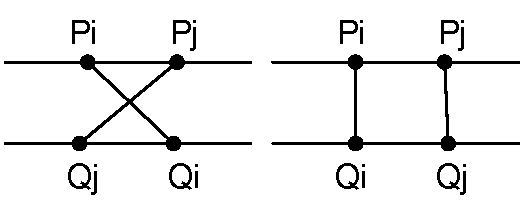
\includegraphics[width=0.25\textwidth]{pb2}
  \caption{Two-node cases of inversion vs intersection}
  \label{fig:pb2}
  \end{figure}

  Summarizing the two cases, we have Total number of intersections $ = $ Total number of inversions, thus the theorem holds. 

  (b)

  Given the conclusion in Problem 1, permutations do not cause the number of inversions to change, this algorithm uses one list as the standard, takes in the other list, and calculates its number of inversions when compared against the standard. The algorithm's given in alg. \ref{alg:number-of-inversions-mergesort}.
  
  \begin{algorithm}[h]
  \caption{Number of inversions for one list against a permutated standard}
  \label{alg:number-of-inversions-mergesort}
    \begin{algorithmic}[1]
    \Function{numberOfInversions}{array}
      \State $n \gets len(array)$
      \If {$n < 2$}
        \State \Return $0$
      \EndIf
      
      \State $l1 \gets numberOfInversions(array[0]..array[n/2])$
      \State $l2 \gets numberOfInversions(array[n/2+1]..array[n])$

      \State \Return $l1 + l2 + countInversions(array, array[0]..array[n/2], array[n/2+1]..array[n])$
    \EndFunction

    \Function{countInversions}{original,l1,l2}
      \State $inversions \gets 0$
      \State $n \gets len(l1)$
      \State $pos \gets 0$

      \While {$l1.hasNext() \vee l2.hasNext()$}
        \If {$l1.hasNext() = false$}
          \State $original[pos] \gets l2.next()$
        \ElsIf {$l2.hasNext() = false$}
          \State $original[pos] \gets l1.next()$
        \ElsIf {$l1.next() < l2.next()$}
          \State $original[pos] \gets l1.next()$
        \Else
          \State $original[pos] \gets l2.next()$
          \State $i \gets n - l2.next()'s \quad position \quad in \quad l1$
          \State $inversions \gets inversions + i$
        \EndIf
        
        \State $pos \gets pos + 1$
      \EndWhile

      \State \Return $inversions$
    \EndFunction

    \end{algorithmic}
  \end{algorithm}
  
  \textbf{Time complexity:} this algorithm adds a constant-time inversion count to a recursive merge sort, thus the complexity is the same as merge sort, which is $O(n\log n)$. In other words, the above described algorithm satisfies $T(n) = 2 \cdot T(\frac{n}{2}) + n$, by Master Theorem case 2, we have $T(n) = O(n\log{n})$.

  \textbf{Correctness:} this algorithm takes over after both arrays are permutated, such that one array is sorted and considered a standard array, and the other array is given as input for counting the number of inversions. 

  This algorithm uses divide and conquer: each time we split the input array into two, if we assume the two sub arrays are sorted and already have their number of inversions counted, the number of inversions of the merged array is the sum of the number of inversions of the two sub arrays, plus the number of inversions introduced by the merge, which is $\sum_{i=1}^{n}{a_i}$, where $n$ is the number of elements in the right array, and $a_i$ is the left array's number of elements that are to the right of the $i^th$ element in the right array, if that element were to be inserted in the left array.

\item[3]{Celebrity iterative}

  Given an incident matrix representation of the graph, the algorithm's given in alg. \ref{alg:celebrity-iterative}. The algorithm takes in an $n \times n$ incident matrix (whose \textit{len} is defined as $n$; and $matrix[i][j] = 1$ means person $i$ knows person $j$), and returns the index of the celebrity if there's one, otherwise returns $-1$. Matrix with less than two persons is considered to not have celebrities.

  (Minor detail: the following algorithm assumes incident matrix index starts from 0)

  \begin{algorithm}[h]
  \caption{Celebrity iterative}
  \label{alg:celebrity-iterative}
    \begin{algorithmic}[1]
    \Function{hasCelebrity}{matrix}
      \State $l \gets len(matrix)$
      \If {$l < 2$}
        \State \Return $-1$
      \EndIf
      \State $i \gets 0$
      \State $j \gets 1$

      \While {$max(i, j) < l$}
        \If {$matrix[i][j] = 1 \wedge matrix[j][i] = 0$}
          \State $i \gets max(i,j) + 1$
        \ElsIf {$matrix[j][i] = 1 \wedge matrix[i][j] = 0$}
          \State $j \gets max(i,j) + 1$
        \Else
          \State $i \gets max(i,j) + 1$
          \State $j \gets max(i,j) + 1$
        \EndIf
      \EndWhile

      \If {$min(i, j) \geq l$}
        \State \Return $-1$
      \EndIf

      \If {$i \geq l$}
        \State \Return $isCelebrity(matrix, j)$
      \Else
        \State \Return $isCelebrity(matrix, i)$
      \EndIf
    \EndFunction

    \Function{isCelebrity}{matrix, i}
      \For {person $p$ in matrix, $p \neq i$}
        \If {$matrix[p][i] = 0 \vee matrix[i][p] = 1$}
          \State \Return $-1$
        \EndIf
      \EndFor
      \State \Return $i$
    \EndFunction
    \end{algorithmic}
  \end{algorithm}

  \textbf{Time complexity:} this algorithm is $O(n)$, where $n$ is the number of persons. In each execution of while, we get rid of at least one person from an arbitrary pair. So the loop's executed at most $n$ times, and each time it executes a constant number of operations. The check for whether the last remaining person is a celebrity or not is also $O(n)$, so the overall algorithm is $O(n)$.

  \textbf{Correctness:} as discussed in class, there is at most one celebrity in a group of people. So each time the algorithm takes a pair of persons, see if they know each other, and remove the one that's definitely not a celebrity (or remove both if neither is a celebrity), and move on until there's only one person left. We then check if that person is a celebrity and returns the result.

\item[4]{Diameter of tree}
  
  (a)

  Define the \textbf{height} of a rooted directed tree as the number of edges on the longest path from the root to a leaf. Algorithm is given in alg \ref{alg:tree-diameter-recursive}.

  \begin{algorithm}[h]
  \caption{Diameter of a rooted directed tree's underlying undirected tree, recursive}
  \label{alg:tree-diameter-recursive}
    \begin{algorithmic}[1]
    \Function{findDiameter}{root}
      \State $heights \gets []$
      \State $diameter \gets 0$
      \State $diameters \gets []$
      \For {\textbf{each} $\{ n | n \in V, (n, root) \in E\}$}
        \State $heights.push(findHeight(n))$
        \State $diameters.push(findDiameter(n))$
      \EndFor
      \If {$len(heights) = 0$}
        \State $diameter \gets 0$
      \ElsIf {$len(heights) = 1$} 
        \State $diameter \gets heights[0] + 1$
      \Else
        \State $diameter \gets 2 + max(heights) + 2^{nd}heighest(heights)$
      \EndIf
      \State \Return $max(diameter, diameters)$
    \EndFunction

    \Function{findHeight}{root}
      \State $queue \gets [root]$
      \State $height \gets 0$
      \While {True}
        \State $nodeCount \gets queue.size()$
        \If {$nodeCount = 0$}
          \State \Return $height$
        \EndIf
        \State $height \gets height + 1$
        \While {$nodeCount > 0$}
          \State $r \gets queue.dequeue()$
          \State $r.visited \gets true$
          \For {\textbf{each} $ \{n | n \in V, (n, r) \in E, n.visited = false\}$}
            \State $queue.enqueue(n)$
          \EndFor
          \State $nodeCount \gets nodeCount - 1$
        \EndWhile
      \EndWhile
    \EndFunction
    \end{algorithmic}
  \end{algorithm}

  \textbf{Correctness:} starting from the root in the tree, diameter is the maximum among the diameters of its sub-trees, and the sum of heights of its two highest sub-trees plus two. Assuming the diameters of its sub-trees are already found, we combine this algorithm with \textit{tree-height} algorithm from last homework, and produce the largest among these values as the diameter of the tree.

  \textbf{Time complexity:} this algorithm is $O(n\log{n})$, where $n$ is the number of nodes in the tree. This algorithm satisfies $T(n, i) = \sum_{i' | (root, i') \in E}{T(n', i')} + n$, where $n$ is the number of nodes that are lower than node $i$, and $n'$ is the number of nodes that are lower than node $i'$. The $+n$ comes from the cost of \textit{findHeight}, which gets called each time we recursively call \textit{findDiameter}. For simplicity, assuming it's a full tree with fanout $k$, we have $T(n) = k \cdot \sum_{T(\frac{n}{k})} + n$. And by Master Theorem case 2, this algorithm is $O(n\log{n})$.

  (b)

  The iterative version of the algorithm is given in alg \ref{alg:tree-diameter-iterative}. Starting from a given root, this algorithm first does a BFS traversal. The last dequeued node is then used as a starting point for the same \textit{findHeight} algorithm used in part (a) and the previous homework.

  \begin{algorithm}[h]
  \caption{Diameter of a rooted directed tree's underlying undirected tree, iterative}
  \label{alg:tree-diameter-iterative}
    \begin{algorithmic}[1]
    \Function{findDiameter}{root}
      \State $queue \gets [root]$
      \While {$queue \neq []$}
        \State $r \gets queue.dequeue()$
        \For {\textbf{each} $ \{n | n \in V, (n, r) \in E, n.visited = false\}$}
          \State $queue.enqueue(n)$
          \State $n.visited \gets true$
        \EndFor
      \EndWhile
      \For {\textbf{each} $ \{n | n \in V\}$}
        \State $n.visited \gets false$
      \EndFor

      \State \Return $findHeight(r)$
    \EndFunction

    \Function{findHeight}{root}
      \State $queue \gets [root]$
      \State $height \gets 0$
      \While {True}
        \State $nodeCount \gets queue.size()$
        \If {$nodeCount = 0$}
          \State \Return $height$
        \EndIf
        \State $height \gets height + 1$
        \While {$nodeCount > 0$}
          \State $r \gets queue.dequeue()$
          \State $r.visited \gets true$
          \For {\textbf{each} $ \{n | n \in V, (n, r) \in E, n.visited = false\}$}
            \State $queue.enqueue(n)$
          \EndFor
          \State $nodeCount \gets nodeCount - 1$
        \EndWhile
      \EndWhile
    \EndFunction

    \end{algorithmic}
  \end{algorithm}
  
  % My previous solution is wrong, key is, root can be any node. So the algorithm should work for arbitrary nodes

  \textbf{Correctness:} starting from the root $r$, after the first BFS, a leaf node $n$ who's farthest away from the $r$ is returned; we want to prove that starting from $n$, we can find the diameter. Idea of the proof centers around the property: for any pair of nodes $(a,b)$, there exists only one path $(a,b)$.

  Assume we have diameter $D = d(s,e)$, case analysis on whether the path $(s,e)$ and path $(r,n)$ share edges or not.

  \begin{itemize}
    \item
    Path $(s,e)$ and path $(r,n)$ do not share edges. Path $(s,n)$ should then contain node $r$. (Otherwise assume that $(s, n)$ and $(r, n)$ first converges at $l, l \neq r$, we have $d(r, n) > d(l, n) \geq d(l,e) \geq d(s,e) = D$, a contradiction with the definition of diameter). Similarly, path $(e,n)$ should contain node $r$, and node $r$ is on path $(s,e)$. Since $d(r,n) \geq max(d(r,s), d(r,e))$, we have $max(d(n,s),d(n,e)) = d(r,n) + max(d(r,s), d(r,e)) \geq d(s,e) = D$. Then we can always find the diameter starting from $n$.

    \item
    Path $(s,e)$ and path $(r,n)$ share a path $(a,b)$. Assume that $a$ being closer to $s$, and $b$ being $e$. We have $d(a,n) \geq d(a,e)$, $d(a,n) \geq d(a,s)$, $d(b,n) \geq d(b,e)$, $d(b,n) \geq d(b,s)$. Thus in case of $a$ being closer to $n$ than $b$ is, we have $D = d(s,e) = d(s,a) + d(a,b) + d(b,e) \leq d(n,a) + d(a,b) + d(b,e) = d(n,e)$; otherwise we have $D = d(s,e) = d(s,a) + d(a,b) + d(b,e) \leq d(s,a) + d(a,b) + d(b,n) = d(n,s)$. Then we can always find the diameter starting from $n$.
  \end{itemize}

  Summarizing both cases, we prove that we can always find the diameter starting from the last node dequeued by BFS started from any node.

  \textbf{Time complexity:} this algorithm is $O(n)$, where $n$ is the number of nodes in the tree, because this algorithm first does BFS which is $O(n)$, then resets the visited flag which is $O(n)$, and finally does \textit{findHeight}, which is also $O(n)$ per the analysis in the previous homework.

\end{description}

\end{document}
